%doc: 2a tramesa revista/revista2n10111rtrimestre/Museu 2n.docx
\begin{news}
{2} %columnes
{El sabor dolç}
{Hi havia una vegada uns nens i nenes de segon de primària que van anar al Museu d’Història de Catalunya per aprendre com l’ésser humà va descobrir el sabor \emph{dolç}}
{Primaria}
{304} %pagesof

\noindent\fbox{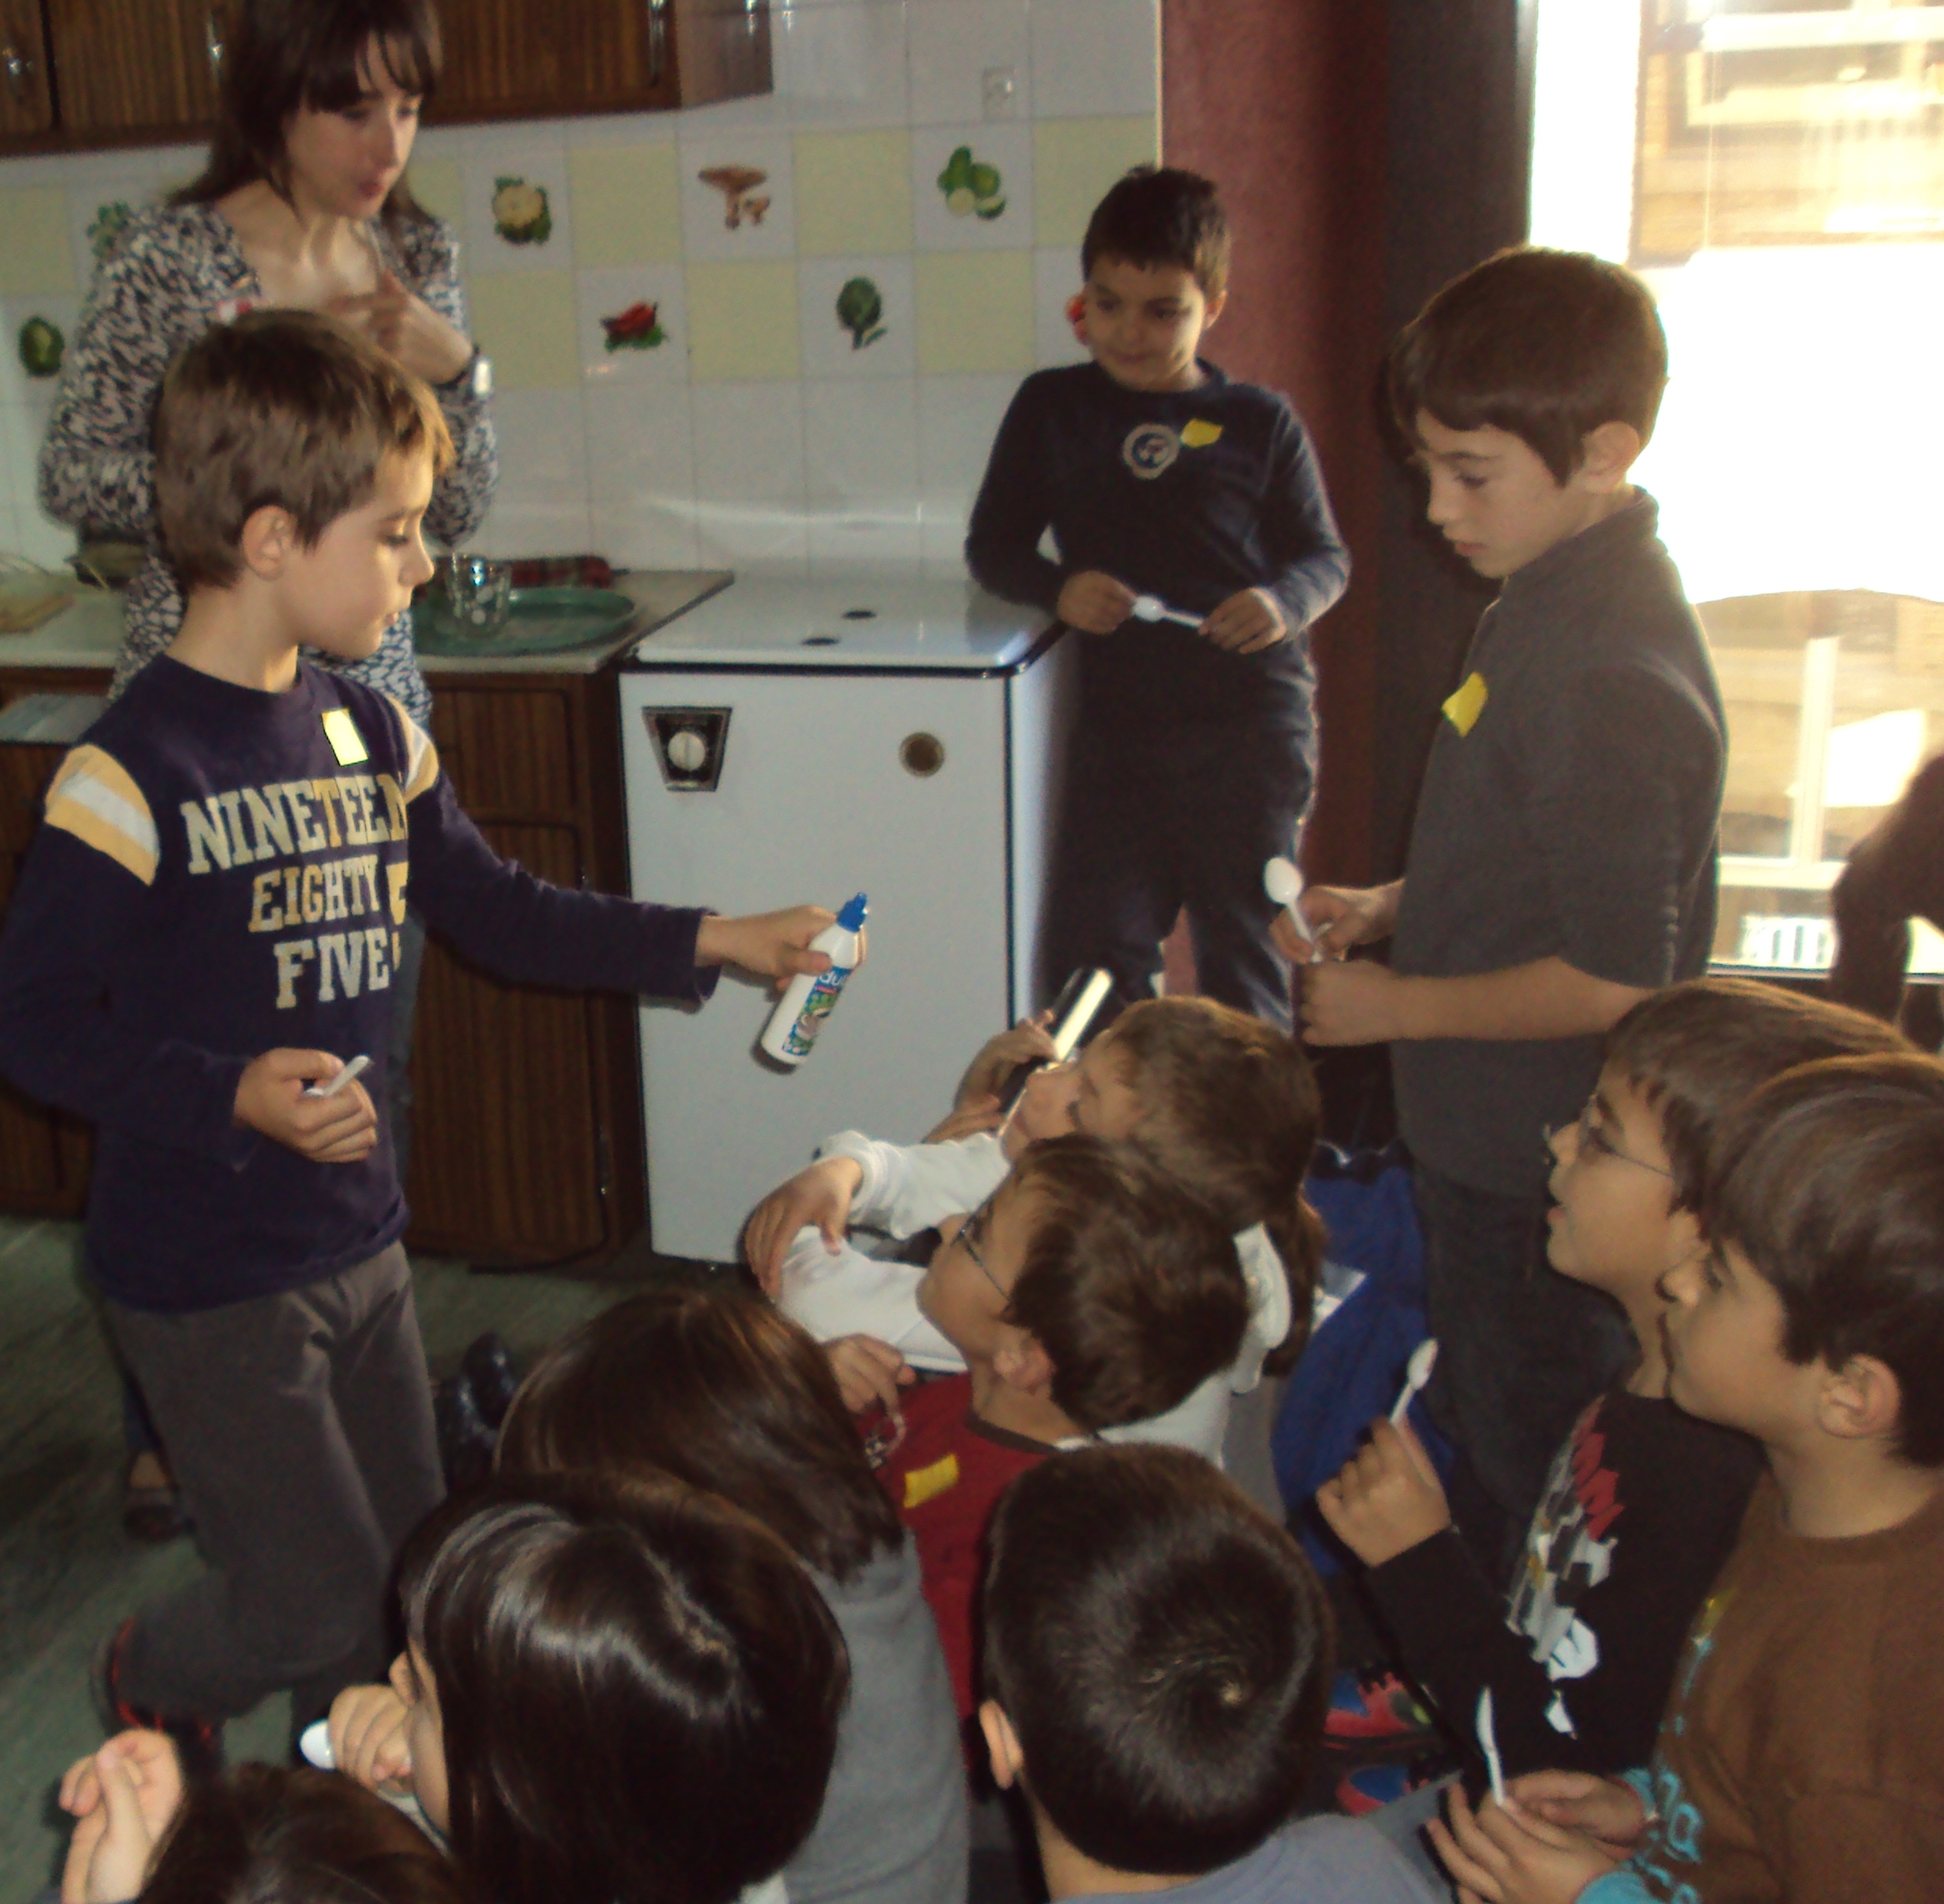
\includegraphics[width=8.5cm,keepaspectratio]{primaria/img/museu_209.jpg}}

Per començar, van anar a la sala de la \emph{Prehistòria} i van aprendre dues paraules noves \emph{Paleolític} i \emph{Neolític}.

Durant aquest temps, els homes i dones van descobrir que alguns aliments eren més dolços que altres. Les fruites que trobaven mentre caminaven pel bosc: maduixetes, groselles, móres, cireretes..., van ajudar a educar el paladar als humans del Paleolític. 

Els homes i les dones del Neolític començaren a conrear els seus aliments, ja no només caçaven com els seus avis, ara ja eren  capaços de tenir animals a casa seva: ovelles, cabres, vaques..., per això podien beure llet.

Continuem la línia del temps, corre el temps, corre... Han passat molts milers d’anys i ens trobem amb els \emph{grecs} i els \emph{romans}. Dues civilitzacions que han estat la base de la nostra cultura. Saben com conservar la carn utilitzant la sal marina, emmagatzemen els cereals, tot ho poden transportar d’un cantó a l’altre,, fins i tot, amb les seves naus, ho poden compartir amb altres contrades llunyanes. Tant els uns com els altres ja poden endolcir els aliments i ja són capaços de fer els seus pastissos  a base de \emph{mel}.

Corre el temps, corre i passem a l’\emph{Edat Mitjana}. Durant aquest temps ens trobem amb un nou poble que ens enriquirà amb la seva cultura, els \emph{àrabs}, que a més d’endolcir amb la mel, utilitzen la melassa treta d’una mena de canya que trinxaven i bullien. La seva rebosteria i varietat de pastissos era molt rica. Nosaltres encara conservem alguns dels seus dolços, per exemple els \emph{torrons},i els \emph{pastissets}.

Corre el temps,  roda que rodaràs i \emph{Cristòfor Colom},  un mariner molt important, amb tres vaixells molt grossos, la Pinta, La Niña i la Santa Maria, creua l’Oceà Atlàntic i ara tenim patates i xocolata i més...\emph{Edat Moderna}.

El temps no para i ens anem fent grans i les persones anem fent més descobriments, les cases són cada cop més còmodes. I les receptes de la cuina més riques i saboroses. Ja tenim \emph{sucre}. Hem aconseguit que  aquella melassa dels àrabs ara sigui un munt de cristallets de color marró, que bo! Amb una mica més de temps també s’aconseguirà treure sucre d’altres productes i fer-lo blanc i líquid, -les gotetes que la mama es posa al cafè- perquè no engreixi tant, i sigui més sa pel nostre cos. Els pastissos, ara a la nostra era, l’\emph{Edat Contemporània}, s’han multiplicat. Tenim llaminadures de moltes menes!! \emph{Atenció!!! Compte amb les càries, Atenció perquè no ens ajuden en el nostre creixement}.

I conte contat ja hem acabat. 
  
\end{news}
